\documentclass[a4paper,11pt]{article}
\usepackage[utf8]{inputenc}
\usepackage{fancyhdr}
\usepackage[pdftex]{graphicx}

\usepackage[spanish]{babel}


\newenvironment{scaption}[1]{\caption{{\small #1}}}{}

\newenvironment{desig}{\begin{list}{}{\setlength{\labelsep}{0cm}\setlength{\labelwidth}{0cm}\setlength{\listparindent}{0cm}\setlength{\rightmargin}{\leftmargin}}}{\end{list}}



\title{Estructura de Módulos del Sistema FG-Tester}
\date{2008}
\author{Pablo Rodriguez Monetti}


\begin{document}
 
\maketitle

\newpage


\begin{figure}
\begin{center}
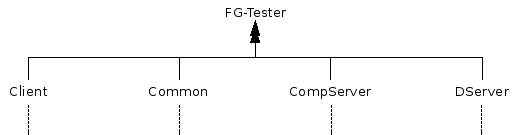
\includegraphics[scale=0.6]{./EstrucModulos01.png}
\end{center}
\caption{Estructura de Módulos (Parte 1).}
\end{figure}


\begin{figure}
\begin{center}
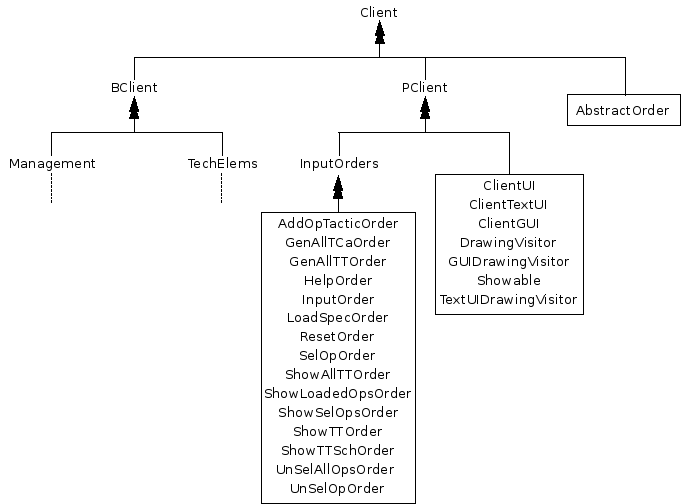
\includegraphics[scale=0.6]{./EstrucModulos02.png}
\end{center}
\caption{Estructura de Módulos (Parte 2).}
\end{figure}


\begin{figure}
\begin{center}
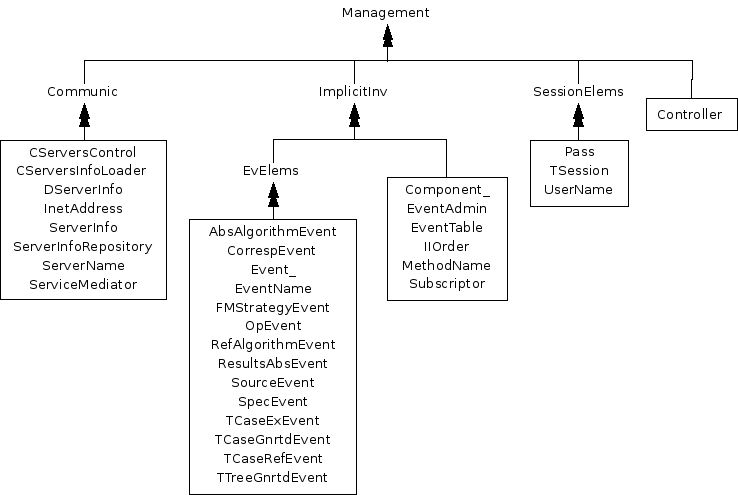
\includegraphics[scale=0.6]{./EstrucModulos03.png}
\end{center}
\caption{Estructura de Módulos (Parte 3).}
\end{figure}


\begin{figure}
\begin{center}
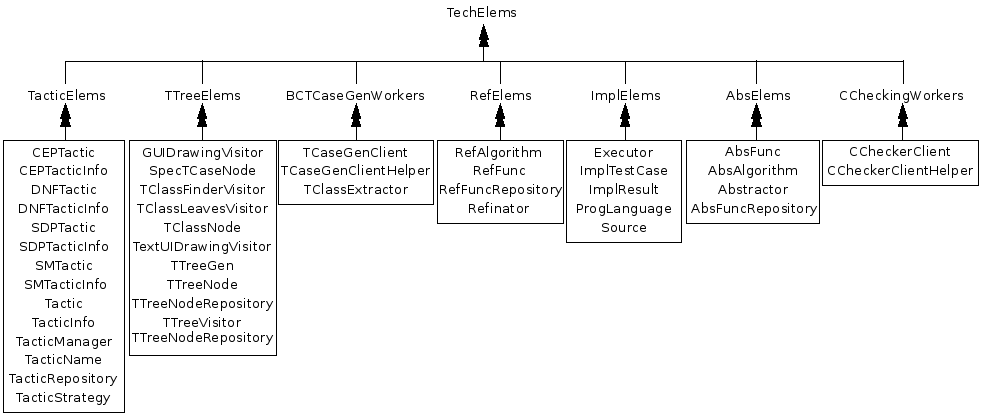
\includegraphics[scale=0.6]{./EstrucModulos04.png}
\end{center}
\caption{Estructura de Módulos (Parte 4).}
\end{figure}


\begin{figure}
\begin{center}
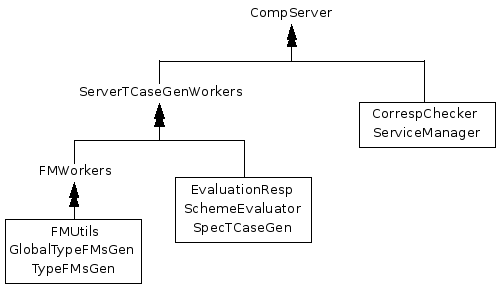
\includegraphics[scale=0.6]{./EstrucModulos05.png}
\end{center}
\caption{Estructura de Módulos (Parte 5).}
\end{figure}


\begin{figure}
\begin{center}
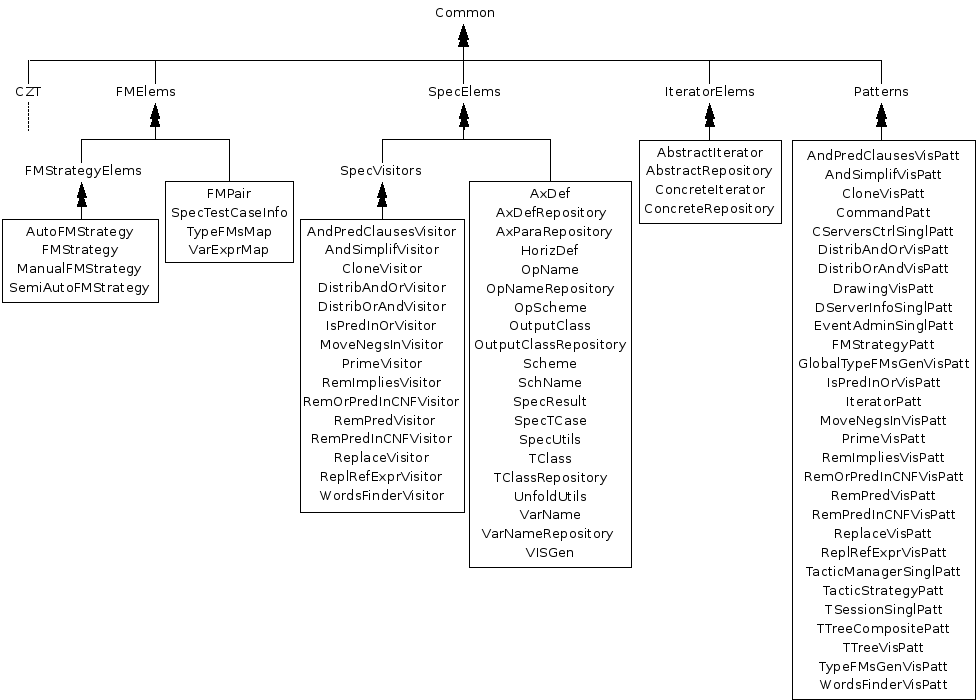
\includegraphics[scale=0.6]{./EstrucModulos06.png}
\end{center}
\caption{Estructura de Módulos (Parte 6).}
\end{figure}


\begin{figure}
\begin{center}
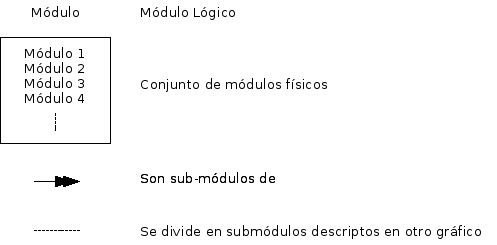
\includegraphics[scale=0.6]{./EstrucModulos00.png}
\end{center}
\caption{Referencias.}
\end{figure}

\end{document}